%%%%%%%%%%%%%%%%%%%%%%%%%%%%%%%%%%%%%%%%
% datoteka diploma-vzorec.tex
%
% vzorčna datoteka za pisanje diplomskega dela v formatu LaTeX
% na UL Fakulteti za računalništvo in informatiko
%
% vkup spravil Gašper Fijavž, december 2010
% 
%
%
% verzija 12. februar 2014 (besedilo teme, seznam kratic, popravki Gašper Fijavž)
% verzija 10. marec 2014 (redakcijski popravki Zoran Bosnić)
% verzija 11. marec 2014 (redakcijski popravki Gašper Fijavž)
% verzija 15. april 2014 (pdf/a 1b compliance, not really - just claiming, Damjan Cvetan, Gašper Fijavž)
% verzija 23. april 2014 (privzeto cc licenca)
% verzija 16. september 2014 (odmiki strain od roba)
% verzija 28. oktober 2014 (odstranil vpisno številko)
% verija 5. februar 2015 (Literatura v kazalu, online literatura)

\documentclass[a4paper, 12pt]{book}
\usepackage{color}
\definecolor{orange}{rgb}{1,0.6,0}
\usepackage[utf8x]{inputenc}   % omogoča uporabo slovenskih črk kodiranih v formatu UTF-8
\usepackage[slovene,english]{babel}    % naloži, med drugim, slovenske delilne vzorce
\usepackage[pdftex]{graphicx}  % omogoča vlaganje slik različnih formatov
\usepackage{fancyhdr}          % poskrbi, na primer, za glave strani
\usepackage{amssymb}           % dodatni simboli
\usepackage{amsmath}           % eqref, npr.
%\usepackage{hyperxmp}
\usepackage[pdftex, colorlinks=true,
						citecolor=black, filecolor=black, 
						linkcolor=black, urlcolor=black,
						pagebackref=false, 
						pdfproducer={LaTeX}, pdfcreator={LaTeX}, hidelinks]{hyperref}

\usepackage{listings}     

%%%%%%%%%%%%%%%%%%%%%%%%%%%%%%%%%%%%%%%%
%	DIPLOMA INFO
%%%%%%%%%%%%%%%%%%%%%%%%%%%%%%%%%%%%%%%%
\newcommand{\ttitle}{Orodje za ročno poravnavo 2D in 3D medicinskih posnetkov}
\newcommand{\ttitleEn}{A tool for manual alignment of 2D and 3D medical recordings}
\newcommand{\tsubject}{\ttitle}
\newcommand{\tsubjectEn}{\ttitleEn}
\newcommand{\tauthor}{Jure Kolenko}
\newcommand{\tkeywords}{Muh keyword1, hue}
\newcommand{\tkeywordsEn}{Muh keyword1, hue}



\usepackage{hyperref}
%%%%%%%%%%%%%%%%%%%%%%%%%%%%%%%%%%%%%%%%
%	HYPERREF SETUP
%%%%%%%%%%%%%%%%%%%%%%%%%%%%%%%%%%%%%%%%
\hypersetup{pdftitle={\ttitle}}
\hypersetup{pdfsubject=\ttitleEn}
\hypersetup{pdfauthor={\tauthor}}
\hypersetup{pdfkeywords=\tkeywordsEn}

%%%%%%%%%%%%%%%%%%%%%%%%%%%%%%%%%%%%%%%%
% postavitev strani
%%%%%%%%%%%%%%%%%%%%%%%%%%%%%%%%%%%%%%%%  

\addtolength{\marginparwidth}{-20pt} % robovi za tisk
\addtolength{\oddsidemargin}{40pt}
\addtolength{\evensidemargin}{-40pt}

\renewcommand{\baselinestretch}{1.3} % ustrezen razmik med vrsticami
\setlength{\headheight}{15pt}        % potreben prostor na vrhu
\renewcommand{\chaptermark}[1]%
{\markboth{\MakeUppercase{\thechapter.\ #1}}{}} \renewcommand{\sectionmark}[1]%
{\markright{\MakeUppercase{\thesection.\ #1}}} \renewcommand{\headrulewidth}{0.5pt} \renewcommand{\footrulewidth}{0pt}
\fancyhf{}
\fancyhead[LE,RO]{\sl \thepage} \fancyhead[LO]{\sl \rightmark} \fancyhead[RE]{\sl \leftmark}



\newcommand{\BibTeX}{{\sc Bib}\TeX}

%%%%%%%%%%%%%%%%%%%%%%%%%%%%%%%%%%%%%%%%
% naslovi
%%%%%%%%%%%%%%%%%%%%%%%%%%%%%%%%%%%%%%%%  


\newcommand{\autfont}{\Large}
\newcommand{\titfont}{\LARGE\bf}
\newcommand{\clearemptydoublepage}{\newpage{\pagestyle{empty}\cleardoublepage}}
\setcounter{tocdepth}{1}	      % globina kazala

%%%%%%%%%%%%%%%%%%%%%%%%%%%%%%%%%%%%%%%%
% konstrukti
%%%%%%%%%%%%%%%%%%%%%%%%%%%%%%%%%%%%%%%%  
\newtheorem{izrek}{Izrek}[chapter]
\newtheorem{trditev}{Trditev}[izrek]
\newenvironment{dokaz}{\emph{Dokaz.}\ }{\hspace{\fill}{$\Box$}}

%%%%%%%%%%%%%%%%%%%%%%%%%%%%%%%%%%%%%%%%%%%%%%%%%%%%%%%%%%%%%%%%%%%%%%%%%%%%%%%
%% PDF-A
%%%%%%%%%%%%%%%%%%%%%%%%%%%%%%%%%%%%%%%%%%%%%%%%%%%%%%%%%%%%%%%%%%%%%%%%%%%%%%%

%%%%%%%%%%%%%%%%%%%%%%%%%%%%%%%%%%%%%%%% 
% define medatata
%%%%%%%%%%%%%%%%%%%%%%%%%%%%%%%%%%%%%%%% 
\def\Title{\ttitle}
\def\Author{\tauthor}
\def\Subject{\ttitleEn}
\def\Keywords{\tkeywordsEn}

%%%%%%%%%%%%%%%%%%%%%%%%%%%%%%%%%%%%%%%% 
% \convertDate converts D:20080419103507+02'00' to 2008-04-19T10:35:07+02:00
%%%%%%%%%%%%%%%%%%%%%%%%%%%%%%%%%%%%%%%% 
\def\convertDate{%
    \getYear
}

{\catcode`\D=12
 \gdef\getYear D:#1#2#3#4{\edef\xYear{#1#2#3#4}\getMonth}
}
\def\getMonth#1#2{\edef\xMonth{#1#2}\getDay}
\def\getDay#1#2{\edef\xDay{#1#2}\getHour}
\def\getHour#1#2{\edef\xHour{#1#2}\getMin}
\def\getMin#1#2{\edef\xMin{#1#2}\getSec}
\def\getSec#1#2{\edef\xSec{#1#2}\getTZh}
\def\getTZh +#1#2{\edef\xTZh{#1#2}\getTZm}
\def\getTZm '#1#2'{%
    \edef\xTZm{#1#2}%
    \edef\convDate{\xYear-\xMonth-\xDay T\xHour:\xMin:\xSec+\xTZh:\xTZm}%
}

\expandafter\convertDate\pdfcreationdate 

%%%%%%%%%%%%%%%%%%%%%%%%%%%%%%%%%%%%%%%%
% get pdftex version string
%%%%%%%%%%%%%%%%%%%%%%%%%%%%%%%%%%%%%%%% 
\newcount\countA
\countA=\pdftexversion
\advance \countA by -100
\def\pdftexVersionStr{pdfTeX-1.\the\countA.\pdftexrevision}


%%%%%%%%%%%%%%%%%%%%%%%%%%%%%%%%%%%%%%%%
% XMP data
%%%%%%%%%%%%%%%%%%%%%%%%%%%%%%%%%%%%%%%%  
\usepackage{xmpincl}
\includexmp{pdfa-1b}

%%%%%%%%%%%%%%%%%%%%%%%%%%%%%%%%%%%%%%%%
% pdfInfo
%%%%%%%%%%%%%%%%%%%%%%%%%%%%%%%%%%%%%%%%  
\pdfinfo{%
    /Title    (\ttitle)
    /Author   (\tauthor)
    /Subject  (\ttitleEn)
    /Keywords (\tkeywordsEn)
    /ModDate  (\pdfcreationdate)
    /Trapped  /False
}


%%%%%%%%%%%%%%%%%%%%%%%%%%%%%%%%%%%%%%%%%%%%%%%%%%%%%%%%%%%%%%%%%%%%%%%%%%%%%%%
%%%%%%%%%%%%%%%%%%%%%%%%%%%%%%%%%%%%%%%%%%%%%%%%%%%%%%%%%%%%%%%%%%%%%%%%%%%%%%%

\begin{document}
\selectlanguage{slovene}
\frontmatter
\setcounter{page}{1} %
\renewcommand{\thepage}{}       % preprecimo težave s številkami strani v kazalu

%%%%%%%%%%%%%%%%%%%%%%%%%%%%%%%%%%%%%%%%
%naslovnica
 \thispagestyle{empty}%
   \begin{center}
    {\large\sc Univerza v Ljubljani\\%
      Fakulteta za računalništvo in informatiko}%
    \vskip 10em%
    {\autfont \tauthor\par}%
    {\titfont \ttitle \par}%
    {\vskip 2em \textsc{DIPLOMSKO DELO\\[2mm]
    UNIVERZITETNI ŠTUDIJSKI PROGRAM PRVE STOPNJE RAČUNALNIŠTVO IN INFORMATIKA}\par}%
    \vfill\null%
    {\large \textsc{Mentor}: doc.\ dr.  Matija Marolt\par}%
    {\vskip 2em \large Ljubljana 2015 \par}%
\end{center}
% prazna stran
\clearemptydoublepage

%%%%%%%%%%%%%%%%%%%%%%%%%%%%%%%%%%%%%%%%
%copyright stran
\thispagestyle{empty}
\vspace*{8cm}
Fakulteta za računalništvo in informatiko podpira javno dostopnost znanstvenih, strokovnih in razvojnih rezultatov. Zato priporoča objavo dela pod katero od licenc, ki omogočajo prosto razširjanje diplomskega dela in/ali možnost nadaljne proste uporabe dela. Ena izmed možnosti je izdaja diplomskega dela pod katero od Creative Commons licenc \href{http://creativecommons.si}{http://creativecommons.si}

Morebitno pripadajočo programsko kodo praviloma objavite pod, denimo, licenco 
\emph{GNU General Public License, različica 3}. Podrobnosti licence so dostopne na spletni strani \href{http://www.gnu.org/licenses/}{http://www.gnu.org/licenses/}.

\begin{center}
\mbox{}\vfill
\emph{Besedilo je oblikovano z urejevalnikom besedil \LaTeX.}
\end{center}
% prazna stran
\clearemptydoublepage

%%%%%%%%%%%%%%%%%%%%%%%%%%%%%%%%%%%%%%%%
% stran 3 med uvodnimi listi
\thispagestyle{empty}
\vspace*{4cm}

\noindent
Fakulteta za računalništvo in informatiko izdaja naslednjo nalogo:
\medskip
\begin{tabbing}
\hspace{32mm}\= \hspace{6cm} \= \kill




Tematika naloge:
\end{tabbing}
Fiddy diddling.
\vspace{15mm}

\vspace{2cm}

% prazna stran
\clearemptydoublepage

%%%%%%%%%%%%%%%%%%%%%%%%%%%%%%%%%%%%%%%%
% izjava o avtorstvu
\vspace*{1cm}
\begin{center}
{\Large \textbf{\sc Izjava o avtorstvu diplomskega dela}}
\end{center}

\vspace{1cm}
\noindent Spodaj podpisani Jure Kolenko sem avtor  diplomskega dela z naslovom:

\vspace{0.5cm}
\emph{Vizualizacija medicinskih podatkov}

\vspace{1.5cm}
\noindent S svojim podpisom zagotavljam, da:
\begin{itemize}
	\item sem diplomsko delo izdelal samostojno pod mentorstvom
		doc.\ dr.\ Matije Marolta,

	\item	so elektronska oblika diplomskega dela, naslov (slov., angl.), povzetek (slov., angl.) ter ključne besede (slov., angl.) identični s tiskano obliko diplomskega dela,
	\item soglašam z javno objavo elektronske oblike diplomskega dela na svetovnem spletu preko univerzitetnega spletnega arhiva.	
\end{itemize}

\vspace{1cm}
\noindent V Ljubljani, dne 24. avgusta 2015 \hfill Podpis avtorja:

% prazna stran
\clearemptydoublepage

%%%%%%%%%%%%%%%%%%%%%%%%%%%%%%%%%%%%%%%%
% zahvala
\thispagestyle{empty}\mbox{}\vfill\null\it%
Thanks Obama.
\rm\normalfont

% prazna stran
\clearemptydoublepage

%%%%%%%%%%%%%%%%%%%%%%%%%%%%%%%%%%%%%%%%
% posvetilo
\thispagestyle{empty}\mbox{}{\vskip0.20\textheight}\mbox{}\hfill\begin{minipage}{0.55\textwidth}%
\normalfont\end{minipage}
Posvetilo.
% prazna stran
\clearemptydoublepage

%%%%%%%%%%%%%%%%%%%%%%%%%%%%%%%%%%%%%%%%
% kazalo
\def\thepage{}% preprecimo tezave s stevilkami strani v kazalu
\tableofcontents{}


% prazna stran
\clearemptydoublepage

%%%%%%%%%%%%%%%%%%%%%%%%%%%%%%%%%%%%%%%%
% seznam kratic

\chapter*{Seznam uporabljenih kratic}

\begin{tabular}{l|l|l}
  %{\bf kratica} & {\bf angleško} & {\bf slovensko} \\ \hline
  % after \\: \hline or \cline{col1-col2} \cline{col3-col4} ...
  %{\bf CA} & classification accuracy & klasifikacijska točnost \\
\end{tabular}



% prazna stran
\clearemptydoublepage

%%%%%%%%%%%%%%%%%%%%%%%%%%%%%%%%%%%%%%%%
% povzetek
\addcontentsline{toc}{chapter}{Povzetek}
\chapter*{Povzetek}
V vzorcu je predstavljen postopek priprave diplomskega dela z uporabo okolja \LaTeX. Vaš povzetek mora sicer vsebovati približno 100 besed, ta tukaj je odločno prekratek.
\bigskip

\noindent\textbf{Ključne besede: } \tkeywords.
% prazna stran
\clearemptydoublepage

%%%%%%%%%%%%%%%%%%%%%%%%%%%%%%%%%%%%%%%%
% abstract
\selectlanguage{english}
\addcontentsline{toc}{chapter}{Abstract}
\chapter*{Abstract}
This sample document presents an approach to typesetting your BSc thesis using \LaTeX. A proper abstract should contain around 100 words which makes this one way too short.
\bigskip

\noindent\textbf{Keywords:} \tkeywordsEn.
\selectlanguage{slovene}
% prazna stran
\clearemptydoublepage

%%%%%%%%%%%%%%%%%%%%%%%%%%%%%%%%%%%%%%%%
\mainmatter
\setcounter{page}{1}
\pagestyle{fancy}

\chapter{Uvod}
\chapter{Metode in orodja}
\section{Java in Eclipse}
Za razvoj programskega dela diplomske naloge sem uporabil programski jezik Java in razvojno okolje Eclipse, saj sem z obema že seznanjen.
\subsection*{Java}
Java je objektno orientiran programski jezik, ki ga je razvilo podjetje Sun Microsystems leta 1995. Osnovan je na jezikoma C in C++, vendar pa je višjenivojski, saj pred uporabnikom skrije različne konstrukte, kot so naprimer kazalci in upravljanje s pomnilnikom. Prevede se v nižjenivojski jezik, ki ga nato tolmači javanski navidezni stroj (angl. Java virtual machine - JVM). To omogoča princip \emph{'napiši enkrat, izvajaj kjerkoli'}, kar je bil eden izmed ciljev razvoja tega programskega jezika.
\subsection*{Eclipse}
Eclipse je odprtokodno integrirano razvojno okolje. V osnovi je namenjeno programiranju Java aplikacij, vendar obstajajo vtičniki tudi za mnoge druge jezike. Prednost uporabe Eclipsa je urejevalnik, ki omogoča samodejno dopolnjevanje izrazov in opozarja na napake, ter razhroščevalnik in prikaz dokumentacije.
\section{Hranjenje mrežnega modela}

Za hranjenje mrežnega modela je uporabljena spremenjena različica standarda Obj datotek \textcolor{orange}{[citat]}, ki ga je razvilo podjetje Wavefront technologies. Standard je odprt in ima široko podporo med orodji za vizualizacijo 3-dimenzionalnih (3D) mrežnih modelov. \textcolor{red}{Standard je tekstoven, tako da so datoteke zlahka berljive, slabost tega pa je večja velikost datotek.}
\renewcommand{\lstlistingname}{Datoteka}
\renewcommand{\lstlistlistingname}{Seznam datotek}
\begin{lstlisting}[captionpos=b, frame=single, caption={Primer obj datoteke, ki predstavlja kvadrat.}]
v -1 -1 0
v 1 -1 0
v -1 1 0
v 1 1 0
vt 0 0 0
vt 1 0 0
vt 0 1 0
vt 1 1 0
vn 0 0 1
vn 0 0 1
vn 0 0 1
vn 0 0 1
f 1/1/1 2/2/2 4/4/4
f 1/1/1 4/4/4 3/3/3
\end{lstlisting}

Različica podpira samo del standarda, in sicer zapis za položaje vozlišč ter definicijo ploskev, ne podpira pa naprimer teksturnih koordinat in normal, saj se v programu ne uporabljajo oziroma se izračunajo.

\textcolor{orange}{Lahko podaš tudi primer zapisa trikotnika ali kakšne druge geometrije}

\section{Aplikacija za vizualizacijo}

Aplikacija je namenjena prikazovanju ožilja pacienta. Model se da poljubno obračati in premikati, lahko pa se ga tudi ogleduje v stereo prikazu. Modeli žil so prebrani iz datotek tipa Obj. 

\begin{figure}
\begin{center}
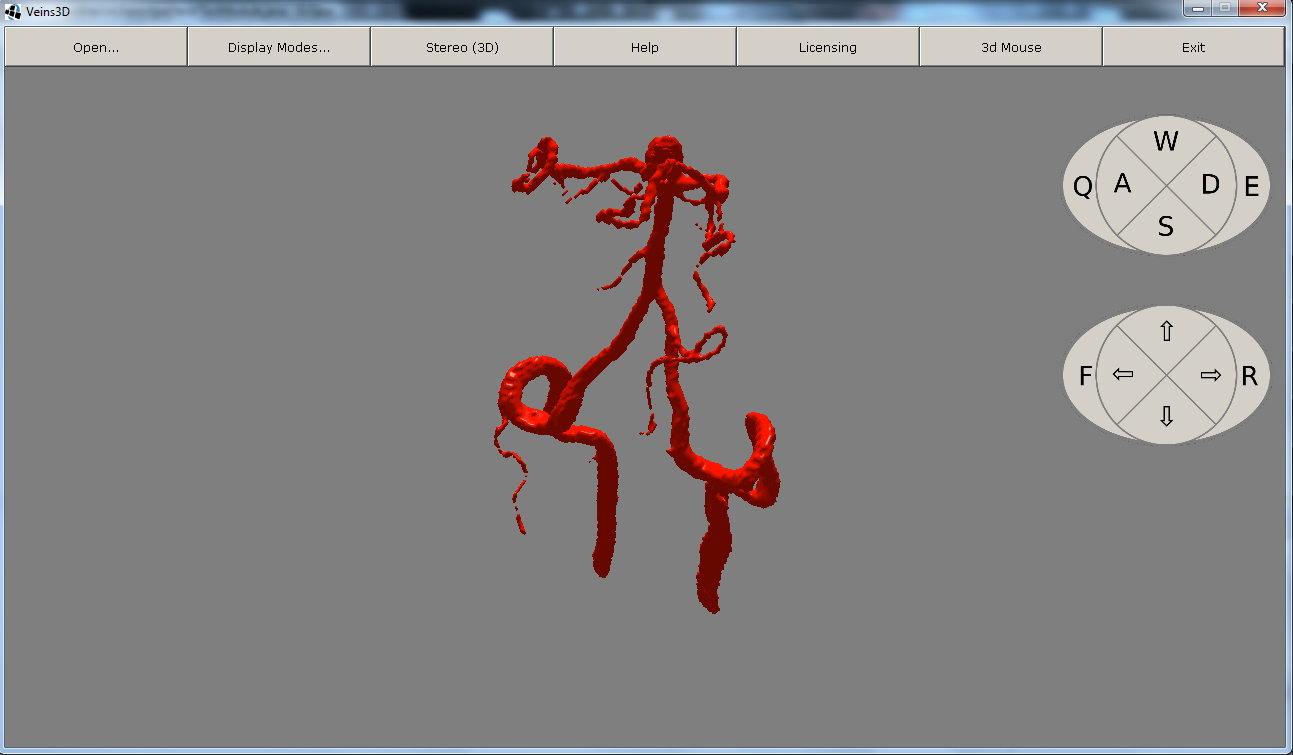
\includegraphics[width=14cm]{aplikacija.png}
\end{center}
\caption{Glavni prikaz aplikacije za vizualizacijo.}
\label{aplikacija}
\end{figure}

\section{Strojno pospešen izris 3D grafike}
Za strojno pospešen izris 3D grafike obstaja več aplikacijskih programerskih vmesnikov, najbolj znana in razširjena pa sta DirectX \textcolor{orange}{[referenca]} in OpenGL  \textcolor{orange}{[referenca]}. DirectX je razvil Microsoft leta 1995 in je namenjen za razvoj aplikacij na operacijskem sistemu Windows, OpenGL pa je leta 1992 razvil Silicon Graphics Inc., sedaj pa ga nadzira neprofitna skupnost Khronos Group, in je namenjen strojno pospešenemu izrisu na večih platformah in v večih jezikih. 

\textcolor{orange}{Tukaj bi bilo smiselno mogoče nekaj več napisati tudi o samem OpenGL-u. Zakaj ga sploh imamo, kaj nam omogoča, ipd.}

V diplomski nalogi sem uporabil odprtokodno knjižnico LWJGL (angl. lightweight java game library), ki omogoča uporabo vmesnika OpenGL.

\textcolor{red}{Opis OpenGLja.}

\section{Projekcija teksture na 3D model}

\textcolor{orange}{Tole potrebuje precej "rewrita". To podpoglavje precej predelaj. Po korakih razloži kako se izvede posamezni korak in pomožnosti dodaj kakšno skico, ki ponazarja kaj se v posameznem koraku zgodi. Prav tako navedi vire, v kolikor si kakšnega uporabljal.}

\textcolor{red}{Projekcija teksture na objekt deluje v treh korakih. Najprej je treba izrisati globinsko sliko iz pogleda projektorja, nato ugotoviti kaj na modelu dejansko zadanejo žarki projektorja, potem pa še pravilno pobarvati dele, ki jih žarki zadanejo.}
\textcolor{red}{\subsection*{Globinska slika}}
\textcolor{red}{Luč se v računalniški grafiki obnaša enako kot kamera. Objekte se, tako kot pri kameri, projecira v pogled luči, nato pa se objekte izriše, pri tem pa se beleži le razdalja do luči oziroma globina najbližjih objektov v vsaki točki. Slika \ref{globinskaslika} je primer izrisa globinske slike.}

\begin{figure}[h]
\begin{center}
\includegraphics[width=12cm, height=10cm, keepaspectratio=true]{Globinska_slika.png}
\end{center}
\caption{Primer globinske slike. Svetlejši kot je piksel, dlje od kamere je objekt.}
\label{globinskaslika}
\end{figure}

\textcolor{red}{\subsection*{Izris objekta s sencami}}
\textcolor{red}{Za izris objekta s sencami, se objekt najprej projecira v pogled kamere in pogled luči. Za vsak delec objekta v pogledu kamere se nato v globinski sliki preveri, če je ta delec viden tudi v pogledu luči. Če je delec viden, se ga osvetli z barvo luči, drugače pa je temnejši. Slika \ref{osencenmodel} je primer tako osenčenega modela.}

\begin{figure}[h]
\begin{center}
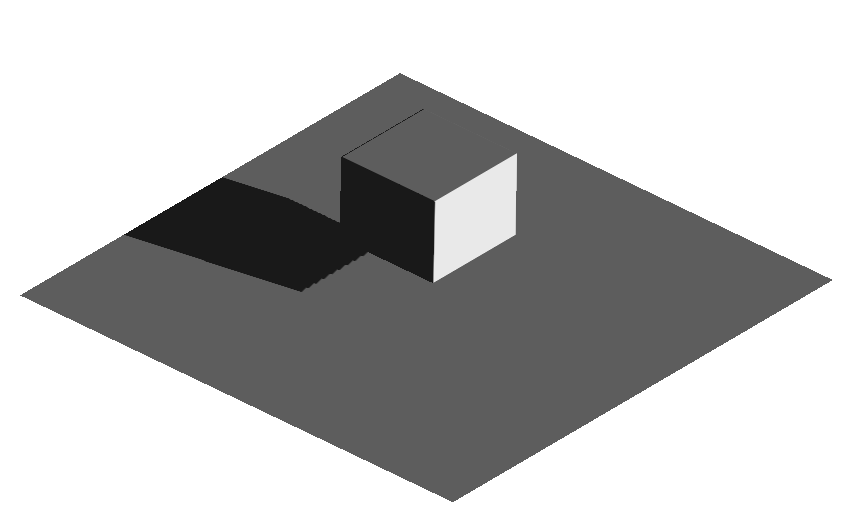
\includegraphics[width=12cm, height=10cm, keepaspectratio=true]{Osencen_model.png}
\end{center}
\caption{Primer osenčenega modela. Luč je na desni strani pred modelom.}
\label{osencenmodel}
\end{figure}

\textcolor{red}{\subsection*{Izris objekta s projecirano sliko}}
\textcolor{red}{Za izris s projekcijo moramo, če je delec viden, izračunati kje v sliki se ta delec nahaja, nato pa namesto bele svetlobe vzeti barvo svetlobe, ki je na tem mestu v sliki. Slika \ref{teksturaprojecirananamodel} je primer izrisa s projecirano sliko, kjer je projecirana slika vijolično-siva šahovnica.}

\begin{figure}[h]
\begin{center}
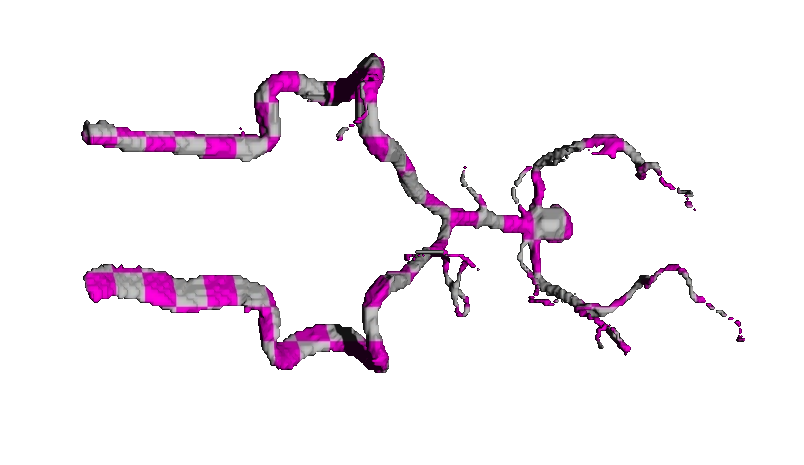
\includegraphics[width=12cm, height=10cm, keepaspectratio=true]{Tekstura_projecirana_na_model.png}
\end{center}
\caption{Primer projekcije teksture na model.}
\label{teksturaprojecirananamodel}
\end{figure}

\textcolor{orange}{Tukaj dodaj še opis podatkov, ki jih bomo uporabljali. Predstaviš da so podatki v OBJ pretvorjeni iz volumetričnih zajetih podatkov kot tudi kakšen je format v katerem so x-ray slike.}

\textcolor{red}{\section{Nabor podatkov}}
\textcolor{red}{3D posnetki so volumetrični posnetki ožilja možganov, narejeni z magnetno resonanco, ki so nato s pomočjo funkcionalnosti že obstoječe aplikacije pretvorjeni v mrežni model, 2D posnetki pa so rentgenski posnetki ožilja shranjeni kot slikovna datoteka tipa jpeg \textcolor{orange}{[citation needed]}.}

\chapter{Implementacija}
\section{Programska ovojnica za LWJGL}

Za lažje delo z OpenGL sem napisal programsko ovojnico, ki temelji na knjižnici LWJGL. OpenGL zahteva veliko knjigovodstva \textcolor{orange}{Ni ravno ustrezen izraz. To opiši.}, saj je treba vsa sredstva, kot so medpomnilniki, senčilniki, teksture in več, ročno uničiti, da se pomnilnik na grafični enoti ne zasiči. Ovojnica to poenostavi tako, da OpenGL sredstva zavije v smiselno poimenovane razrede. Ovojnica nudi tudi transformacije med kvaternioni in evklidskimi koti in razrede za transformacije in kamere.

\subsection*{Medpomnilniki}

Prenašanje podatkov na grafično enoto in z nje v OpenGL poteka prek medpomnilnikov \textcolor{orange}{Povej kateri vsi medpomnilniki obstajajo in za kaj se uporabljajo}. Ovojnica podpira medpomnilnike za sezname, ki se uporabljajo za prenašanje podatkov kot so položaji oglišč, normale v ogliščih in teksturne koordinate, medpomnilnike za elemente, ki grafični enoti povedo iz katerih oglišč so sestavljene ploskve, ter medpomnilnike za okvirje (angl. frame), ki hranijo slike za izris. \textcolor{orange}{To raje razdelaj po točkah, kjer za vsako točko opišeš kaj posamezna vrsta medpomnilnikov hrani.}

\subsection*{Senčilniki}

\textcolor{orange}{V katerem jeziku se pišejo. Dobro bi bilo omeniti, da senčilniki nadomestijo del fiksnega cevovoda in katerega.}

Senčilniki so podprogrami za izris, ki jih mora napisati uporabnik. V starejših verzijah se je uporabljal fiksen cevovod, ki pa je okornejši in manj zmogljiv od uporabniških programov. Ovojnica podpira pet vrst senčilnikov, in sicer senčilnike za oglišča (angl. vertex shader), za geometrijo (geometry), za drobce (fragment) in za deljenje (tesselation), obstaja pa še senčilnik za izračunavanje (compute shader), ki pa ni podprt. Senčilniki se združujejo v programe, ki tvorijo fleksibilen cevovod za izris.
\textcolor{red}{
OpenGL senčilniki se pišejo v jeziku GLSL (angl. OpenGL Shading Language). GLSL je osnovan na jeziku C in omogoča prenosljivost med operacijskimi sistemi in različnimi proizvajalci strojne opreme. }
\subsection*{Teksture}

Teksture v OpenGL so objekti, ki vsebujejo eno ali več slik, ter so uporabni kot vir slikovnih podatkov v senčilnikih ali kot tarča za izris v medpomnilnikih za okvirje. Ker je inicializacija teksture v OpenGL precej kompleksna, ovojnica poskrbi za inicializacijo osnovnih parametrov.

\subsection*{Točkovni nizi}

Točkovni nizi (angl. vertex array object) so OpenGL objekti, ki hranijo stanje potrebno za izris objektov. Hranijo le stanje, ne pa tudi samih podatkov, to je reference na medpomnilnike in obliko podatkov v teh medpomnilnikih, ne pa tudi samih podatkov iz medpomnilnikov. Prednost se kaže v hitrosti in velikosti kode, saj je potrebno veliko manj sprememb stanja.

\subsection*{Transformacija}

\textcolor{orange}{Mogoče bi bilo smiselno kaj več o samih transformacijah napisati v predhodnjem poglavju.}

Transformacija (angl. transform) je razred, ki je namenjen hranjenju transformacije objekta, to je rotacija, položaj in velikost. Položaj in velikost sta predstavljena kot vektorja dolžine 3, rotacija pa kot kvaternion. Podprte so rotacije in premiki v lokalnem ter globalnem koordinatnem sistemu, ter rotacije v poljubnem sistemu. Razred vsebuje tudi funkcije za pretvorbo iz kvaternionov v eulerjeve kote, za izračun transformacijske matrike iz stanja transformacije, ter za izračun kvaterniona iz rotacijske matrike.

(Formule za pretvorbe?)

Kot posebna transformacija se obravnava tudi kamera, le da so pri kameri premiki ravno obrnjeni, ima pa še dodatne parametre za pogled kamere. Podprti sta dve vrsti kamere: perspektivna in vzporedna.
\textcolor{red}{\subsection*{Izjeme}}
\textcolor{red}{Ovojnica podpira več vrst izjem. OpenGL sam ne ustavi izvajanja programa ob napaki, vendar pa je izris nepravilen, zato ob nekaterih operacijah ovojnica preverja, če je na grafični enoti vse v redu. Izjeme se lahko prožijo, ko se senčilnik ne prevede pravilno, ko se program ne poveže pravilno ali ko se medpomnilnik za okvirje ne inicializira pravilno.
}

\subsection*{Ostalo}

Poleg že naštetega ovojnica vsebuje še funkcijo za razhroščevanje, ki napake, ki jih vrača OpenGL, pretvori v berljive nize ter izpiše vrstico v kateri je bila funkcija klicana, kar močno olajša iskanje napak.

\textcolor{orange}{Dobro bi bilo dodati neko shemo tvoje ovojnice, kjer se vidi iz katerih komponent je sestavljena.}

\section{Samostojna aplikacija}

Funkcionalnost orodja sem najprej implementiral kot samostojno aplikacijo, saj je tako lažje preveriti pravilnost delovanja. Aplikacija nima uporabniškega vmesnika, implementiran pa je le osnovni uporabniški nadzor, saj služi le kot primer delovanja, ne pa tudi dejanski uporabi. Sestavljena je iz testnega razreda, razreda ki implementira dejansko funkcionalnost in razredov za branje Obj datotek, ki pa niso uporabljeni v končni aplikaciji, saj ima ta svoj bralnik. Posnetki se v samostojni aplikaciji naložijo avtomatsko iz testnih datotek.

(SLIKA)

\subsection*{Premikanje pogleda}

Aplikacija podpira dva pogleda, pogled iz kamere ter pogled iz projektorja \textcolor{orange}{Kaj je en, kaj je drug, kakšna je razlika, morda skica}. Pogled iz projektorja je namenjen poravnavi 2D in 3D posnetkov, saj je v tem pogledu 2D posnetek pri miru, premika pa se le 3D posnetek. Nepremičnost posnetka v tem pogledu je doseženo s tem, da se pogled in pravokotnik, na katerem je posnetek, obračata in premikata za iste vrednosti. 
\textcolor{orange}{Tole je potrebno opisati na bolj razumljiv način.}

\subsection*{2D posnetek}

Dvo dimenzionalni posnetek je rentgenska slika ožilja. Slika se projecira na pravokotnik, ki je prilagojen velikosti slike. Sliko se da v prostoru rotirati neodvisno od modela, kar služi poravnavi, ko pa sta model in slika poravnana, pa se lahko rotira skupaj z modelom.

\subsection*{3D posnetek}

Tri dimenzionalni posnetek je mrežni model ožilja, naložen iz Obj datoteke. 3D posnetek se sam po sebi se ne premika, premika se le kamera, kar pa da uporabniku podoben vtis.

\section{Integracija v aplikacijo za vizualizacijo}

Za konec sem funkcionalnost integriral še v aplikacijo za vizualizacijo. Poleg funkcionalnosti samostojne aplikacije je bilo potrebno zagotoviti, da se modul obnaša enako kot že obstoječa aplikacija, kar pa ni bilo čisto mogoče, saj modul uporablja drugačno vrsto kamere kot preostala aplikacija. 

\subsection*{Premikanje pogleda}

Model žil se premika enako kot v že obstoječi aplikaciji, s smernimi tipkami za premik levo, desno, naprej in nazaj ter s tipkama 'r' in 'f' za gor in dol. Obrača se s tipkami 'w', 'a', 's', 'd', 'q' in 'e' ter z miško, tako da se lev miškin gumb drži nad objektom in miško premika. Premikanje z miško je, podobno kot v že obstoječi aplikaciji, narejeno s projekcijo kazalca na navidezno kroglo okoli modela, vendar pa je zaradi drugačne vrste kamere izračun preseka drugačen. (*matematika za izračunom*) 


\textcolor{red}{\subsection*{Nalaganje datotek}}
\textcolor{red}{Funkcionalnost za nalaganje datotek je obstajala že v osnovni aplikaciji. Uporabnik s pritiskom na gumb \emph{'odpri'} dobi pojavno okno, v katerem izbira datoteke. Podprti formati so bili mhd za volumetrične datoteke, ter obj za mrežne modele. Moral sem dodati še možnost za nalaganje slikovnih datotek v standardnih formatih jpeg \textcolor{orange}{[citation needed]} in png \textcolor{orange}{[citation needed]}. Java podpira ta dva formata v svoji standardni knjižnici, tako da je bila implementacija preprosta.}

\textcolor{orange}{Manjka ti še predstavitev osnovne aplikacije in predstavitev modulov, ki si jih adaptiral, uporabljal pri svojem delu.}


\chapter{Zaključek}
Ful sm zadovoljen, huehuehue.
\end{document}
